\documentclass[conference]{IEEEtran}
\usepackage{amsmath,amssymb,amsthm}
\usepackage{graphicx}
\usepackage{algorithm}
\usepackage{algpseudocode}
\usepackage{url}
\usepackage{hyperref}

\newtheorem{theorem}{Theorem}
\newtheorem{lemma}{Lemma}
\newtheorem{proposition}{Proposition}
\newtheorem{corollary}{Corollary}
\newtheorem{definition}{Definition}
\newtheorem{remark}{Remark}

\begin{document}

\title{Learning High-Threshold Heterogeneous Networks Through Opinion Dynamics}

\author{
\IEEEauthorblockN{Claude Sonnet 4.5}
\IEEEauthorblockA{Independent Research\\
\texttt{claude@anthropic.ai}}
}

\maketitle

\begin{abstract}
We study the problem of learning social network structure when agents exhibit heterogeneous resistance to opinion change, focusing on the regime of \emph{high-threshold} or stubborn agents. Extending prior work on synchronous majority dynamics, we introduce threshold-heterogeneous networks where each agent has an individual threshold $\tau_i \in [\tau_{\min}, 1)$ determining their susceptibility to influence. For networks where $\tau_{\min} \geq 1 - 1/n$, we prove that learning network topology and identifying threshold intervals requires $O(n^2 + n \log n)$ observations and $O(n^3)$ interventions. Our key technical contribution is a two-phase algorithm that resolves the threshold-structure coupling: Phase 1 learns structure using extreme configurations that work for high-threshold agents, while Phase 2 identifies which of $k_i$ discrete intervals contains each agent's threshold via binary search. With $k_i$ influencers, thresholds are characterized up to precision $1/k_i$, with maximum error $1/(2k_i)$. Numerical experiments validate our theoretical bounds, demonstrating >95\% structure learning accuracy. We discuss why the high-threshold restriction is necessary and outline extensions to broader threshold regimes.
\end{abstract}

\begin{IEEEkeywords}
Social Networks; Opinion Dynamics; Heterogeneous Thresholds; Network Learning; High-Threshold Agents
\end{IEEEkeywords}

\section{Introduction}
\label{sec:introduction}

The inference of social network structure through observed opinion dynamics has emerged as a fundamental problem in computational social choice and multi-agent systems \cite{kempe2003maximizing,netrapalli2012learning}. Recent work by Chistikov et al.~\cite{chistikov2020convergence} established that learning network topology under synchronous majority dynamics requires polynomial observation and intervention budgets. However, their framework assumes homogeneous agent behavior—all agents follow the same update rule with identical thresholds for opinion change.

This assumption is unrealistic in many practical scenarios. Individuals exhibit varying degrees of resistance to persuasion, stubbornness, or susceptibility to peer influence \cite{granovetter1978threshold}. Consider political campaigns targeting skeptical voters, public health initiatives promoting vaccination among resistant populations, or marketing strategies facing brand-loyal consumers. Understanding both \emph{who influences whom} and \emph{how much influence is needed} is crucial for effective intervention.

\subsection{The Challenge of Threshold Heterogeneity}

Extending network learning to heterogeneous thresholds introduces a fundamental challenge: a \emph{threshold-structure coupling}. To learn network structure (which edges exist), one typically creates opinion configurations where agents are "balanced" between changing and not changing. But determining what "balanced" means requires knowing the agent's threshold. Conversely, to identify an agent's threshold, one must know which other agents influence it—requiring knowledge of the network structure.

This circular dependency makes naive approaches fail. Our contribution is to break this coupling through a novel technique using \emph{extreme opinion configurations} that work regardless of threshold value—provided thresholds lie in a restricted but practically relevant regime.

\subsection{High-Threshold Networks}

We focus on \emph{high-threshold} networks where agents are relatively stubborn: each agent $i$ has threshold $\tau_i \geq \tau_{\min}$ for some $\tau_{\min}$ close to 1. This models scenarios where:
\begin{itemize}
\item Voters require overwhelming evidence to change political affiliation
\item Consumers resist switching brands without strong incentives  
\item Community members maintain traditions unless broad consensus emerges
\end{itemize}

The restriction $\tau_{\min} \geq 1 - 1/n$ (where $n$ is the number of agents) is sufficient for our learning algorithm, and captures agents who change opinion only when an overwhelming majority of their influencers disagree.

\subsection{Our Contributions}

\begin{enumerate}
\item \textbf{Framework}: We formalize threshold-heterogeneous networks with individual thresholds $\tau_i \in [\tau_{\min}, 1)$ (Definition~\ref{def:threshold_network}).

\item \textbf{Theoretical Results}: For high-threshold networks ($\tau_{\min} \geq 1 - 1/n$), we prove that learning structure and identifying threshold intervals requires $O(n^2 + n \log n)$ observations and $O(n^3)$ interventions (Theorem~\ref{thm:main_learning}).

\item \textbf{Algorithmic Solution}: We resolve the threshold-structure coupling through extreme configurations: configurations where \emph{all} potential influencers disagree, causing behavior that depends on edge existence regardless of threshold value (Lemma~\ref{lem:extreme_config}).

\item \textbf{Precision Analysis}: With $k_i$ influencers, agent $i$'s threshold is characterized to one of $k_i$ discrete intervals with maximum error $1/(2k_i)$ (Lemma~\ref{lem:threshold_detection}).

\item \textbf{Experimental Validation}: We demonstrate >95\% structure learning accuracy and confirm discretization bounds on high-threshold networks (Section~\ref{sec:experiments}).
\end{enumerate}

\begin{table}[t]
\centering
\caption{Complexity comparison: homogeneous vs. high-threshold heterogeneous networks.}
\label{tab:complexity}
\begin{tabular}{|l|c|c|}
\hline
\textbf{Setting} & \textbf{Observations} & \textbf{Interventions} \\
\hline
Homogeneous \cite{chistikov2020convergence} & $O(n^2)$ & $O(n^3)$ \\
\hline
High-threshold (this work) & $O(n^2 + n \log n)$ & $O(n^3)$ \\
\hline
\end{tabular}
\end{table}

Our results show that threshold heterogeneity adds tractable complexity (additive $O(n \log n)$ observations) rather than fundamentally changing the learning problem, but only within the high-threshold regime where extreme configurations provide threshold-independent information. Table~\ref{tab:complexity} summarizes the complexity comparison.

\subsection{Related Work}

Our work extends the framework of Chistikov et al.~\cite{chistikov2020convergence}, who studied learning under homogeneous majority dynamics. Influence maximization with known structure has been extensively studied \cite{kempe2003maximizing,bredereck2017manipulating}, but learning unknown networks remains less explored.

Network inference from cascade dynamics \cite{netrapalli2012learning,gomez2010inferring} typically assumes knowledge of infection times rather than opinion states. Heterogeneous thresholds appear in models of complex contagions \cite{granovetter1978threshold}, but not from a network learning perspective. We bridge this gap by analyzing how threshold diversity affects learnability.

\section{Preliminaries}
\label{sec:preliminaries}

\subsection{Threshold-Heterogeneous Networks}

We build on the framework of Chistikov et al.~\cite{chistikov2020convergence} for binary opinion dynamics.

\begin{definition}[Threshold-Heterogeneous Social Network]
\label{def:threshold_network}
A threshold-heterogeneous social network is a tuple $(N, G, \tau, \ell)$ where:
\begin{itemize}
\item $N = \{1, \ldots, n\}$ is a finite set of agents,
\item $G \subseteq N \times N$ is a directed graph with no self-loops,
\item $\tau : N \to [\tau_{\min}, 1)$ assigns each agent a threshold, where $\tau_{\min} \geq 1 - 1/n$,
\item $\ell : N \to \{0, 1\}$ is a binary opinion labeling.
\end{itemize}
For agent $i \in N$, we denote $G^{-1}_i = \{j \in N : (j, i) \in G\}$ (influencers of $i$) and $k_i = |G^{-1}_i|$ (in-degree).
\end{definition}

The threshold $\tau_i$ represents agent $i$'s resistance to change. An agent with $\tau_i$ near 1 is highly stubborn. The restriction $\tau_{\min} \geq 1 - 1/n$ ensures $\tau_i \geq 1 - 1/n > 1 - 1/k_i$ for all $i$ (since $k_i \leq n-1$), which is crucial for our learning algorithm.

\begin{definition}[Threshold-Based Opinion Update]
\label{def:threshold_update}
Given $(N, G, \tau, \ell)$, the opinion update produces $\ell^+ : N \to \{0, 1\}$ where:
\[
\ell^+(i) = \begin{cases}
1 - \ell(i) & \text{if } k_i > 0 \text{ and } \frac{|D^{-1}_i|}{k_i} > \tau_i, \\
\ell(i) & \text{otherwise},
\end{cases}
\]
where $D^{-1}_i = \{j \in G^{-1}_i : \ell(j) \neq \ell(i)\}$ (disagreeing influencers).
\end{definition}

The majority rule corresponds to $\tau_i = 0.5$. Our high-threshold regime requires $\tau_i \geq 1 - 1/n$, typically $\tau_i \in [0.80, 0.95]$ for small $n$.

\subsection{The Learning Problem}

\begin{definition}[Exact Learning with Threshold Intervals]
\label{def:exact_learning_threshold}
The campaigner \emph{exactly learns} $(G, \tau)$ if she can infer the edge set $G$ with certainty and, for each agent $i$ with $k_i > 0$ influencers, identify which interval $[\ell/k_i, (\ell+1)/k_i)$ contains $\tau_i$ for some $\ell \in \{0, 1, \ldots, k_i-1\}$.
\end{definition}

The campaigner has budgets $Obs$ (observations) and $Int$ (interventions). Each opinion diffusion step costs one observation; setting agent $i$'s opinion costs one intervention.

\section{Main Results}
\label{sec:results}

\subsection{Breaking the Threshold-Structure Coupling}

The key challenge is that learning structure typically requires knowing thresholds (to create "balanced" states), while identifying thresholds requires knowing structure (to identify influencers). We resolve this through \emph{extreme configurations}.

\begin{lemma}[Extreme Configuration Test for High-Threshold Agents]
\label{lem:extreme_config}
Let $(N, G, \tau)$ be a threshold-heterogeneous network with $\tau_i \in [\tau_{\min}, 1)$ where $\tau_{\min} \geq 1 - 1/n$. Consider agent $i$ and candidate influencer $j \neq i$. Create two opinion states:
\begin{enumerate}
\item $\ell_{\text{all}}$: Agent $i$ has opinion 1, all others have opinion 0
\item $\ell_{\text{-j}}$: Agent $i$ has opinion 1, agent $j$ has opinion 1, all others have opinion 0
\end{enumerate}
Let $\ell^+_{\text{all}}$ and $\ell^+_{\text{-j}}$ be the resulting updates. Then:
\[
j \in G^{-1}_i \iff \left(\ell^+_{\text{all}}(i) \neq \ell_{\text{all}}(i) \text{ and } \ell^+_{\text{-j}}(i) = \ell_{\text{-j}}(i)\right)
\]
\end{lemma}

\begin{proof}
We analyze agent $i$'s behavior in both configurations.

\textbf{Configuration $\ell_{\text{all}}$}: All agents except $i$ have opinion 0, while $i$ has opinion 1. Thus every influencer of $i$ disagrees, giving disagreement fraction $k_i/k_i = 1$. Since $\tau_i < 1$, we have $1 > \tau_i$, so agent $i$ changes opinion: $\ell^+_{\text{all}}(i) = 0 \neq \ell_{\text{all}}(i)$.

\textbf{Configuration $\ell_{\text{-j}}$}: Agents $i$ and $j$ have opinion 1, all others have opinion 0.

\textbf{Case 1}: $j \in G^{-1}_i$ (j is an influencer).
Now only $k_i - 1$ influencers disagree, giving fraction $(k_i - 1)/k_i$. By our restriction, $\tau_i \geq \tau_{\min} \geq 1 - 1/n > 1 - 1/k_i = (k_i-1)/k_i$. Therefore $(k_i-1)/k_i < \tau_i$, so agent $i$ does \emph{not} change: $\ell^+_{\text{-j}}(i) = \ell_{\text{-j}}(i)$.

\textbf{Case 2}: $j \notin G^{-1}_i$ (j is not an influencer).
Changing $j$'s opinion doesn't affect agent $i$'s influencers. The disagreement fraction remains $k_i/k_i = 1 > \tau_i$, so agent $i$ still changes: $\ell^+_{\text{-j}}(i) = 0 \neq \ell_{\text{-j}}(i)$.

Thus: $j \in G^{-1}_i$ iff agent $i$ changes in $\ell_{\text{all}}$ but not in $\ell_{\text{-j}}$.
\end{proof}

\begin{remark}
The condition $\tau_i \geq 1 - 1/k_i$ is \emph{necessary}. For counterexample: if $k_i = 5$ and $\tau_i = 0.7$, then $(k_i-1)/k_i = 0.8 > 0.7$, so agent $i$ changes in \emph{both} configurations regardless of whether $j$ is an influencer, making the test fail.
\end{remark}

This lemma provides threshold-independent edge detection in the high-threshold regime. The key insight: fraction 1 (all influencers disagree) exceeds any threshold $\tau_i < 1$, while fraction $(k_i-1)/k_i$ falls below high thresholds $\tau_i \geq 1 - 1/k_i$.

\subsection{Threshold Interval Identification via Binary Search}

Once structure is known, thresholds can be characterized to discrete intervals efficiently.

\begin{lemma}[Threshold Interval Identification for Known Structure]
\label{lem:threshold_detection}
Let agent $i$ have $k_i = |G^{-1}_i|$ known influencers. Identifying which interval $[\ell/k_i, (\ell+1)/k_i)$ contains $\tau_i$ (for $\ell \in \{0, 1, \ldots, k_i-1\}$) requires at most $\lceil \log_2(k_i) \rceil$ observations.
\end{lemma}

\begin{proof}
With $k_i$ influencers, agent $i$ experiences $k_i+1$ discrete disagreement fractions: $\{0, 1/k_i, \ldots, k_i/k_i\}$. These partition $[0,1]$ into $k_i$ intervals (excluding the boundary case $\tau_i = 1$). Agent $i$'s behavior when presented with disagreement fraction $m/k_i$ reveals whether $\tau_i < m/k_i$ or $\tau_i \geq m/k_i$.

Binary search proceeds as:
\begin{enumerate}
\item Set $\lceil k_i/2 \rceil$ influencers to disagree with agent $i$
\item Observe whether $i$ changes opinion
\item Update search bounds based on result
\item Recurse until interval identified
\end{enumerate}

Binary search over $k_i \leq n-1$ intervals requires $\lceil \log_2(k_i) \rceil \leq \lceil \log_2 n \rceil$ observations.
\end{proof}

\begin{remark}[Precision vs. In-Degree]
\label{rem:precision}
The algorithm identifies threshold intervals, not exact thresholds. With $k_i$ influencers, precision is limited to $\Delta\tau = 1/k_i$. The midpoint estimate has maximum error $1/(2k_i)$. Dense networks or high-degree nodes enable finer-grained threshold characterization; sparse networks yield coarser intervals.
\end{remark}

\subsection{Joint Learning of Structure and Threshold Intervals}

\begin{theorem}[Learning High-Threshold Heterogeneous Networks]
\label{thm:main_learning}
Let $(N, G, \tau)$ be a threshold-heterogeneous network with $n$ agents and $\tau_i \in [\tau_{\min}, 1)$ where $\tau_{\min} \geq 1 - 1/n$. The campaigner can exactly learn $G$ and identify threshold intervals containing each $\tau_i$ using:
\begin{itemize}
\item $O(n^2 + n \log n)$ observations, and
\item $O(n^3)$ interventions.
\end{itemize}
\end{theorem}

\begin{proof}
The learning strategy has two phases for each agent $i \in N$:

\textbf{Phase 1: Structure Learning (Threshold-Independent).} For each potential influencer $j \in N \setminus \{i\}$:
\begin{enumerate}
\item Apply Lemma~\ref{lem:extreme_config} by creating configurations $\ell_{\text{all}}$ and $\ell_{\text{-j}}$
\item Observe two opinion updates to test if $j \in G^{-1}_i$
\item Each configuration requires setting $O(n)$ agent opinions
\end{enumerate}

Testing $n-1$ candidates for agent $i$: $2(n-1) = O(n)$ observations, $O(n^2)$ interventions.
For all $n$ agents: $O(n^2)$ observations, $O(n^3)$ interventions.

\textbf{Phase 2: Threshold Interval Identification.} Once $G^{-1}_i$ is known for agent $i$:
\begin{enumerate}
\item Apply Lemma~\ref{lem:threshold_detection} via binary search
\item Requires $\lceil \log_2(k_i) \rceil \leq \lceil \log_2 n \rceil$ observations
\item Each observation requires $O(n)$ interventions to set configuration
\end{enumerate}

For all $n$ agents: $O(n \log n)$ observations, $O(n^2 \log n)$ interventions.

\textbf{Total Budget:}
\begin{align*}
\text{Observations} &= O(n^2) + O(n \log n) = O(n^2 + n \log n) \\
\text{Interventions} &= O(n^3) + O(n^2 \log n) = O(n^3)
\end{align*}
\end{proof}

\begin{corollary}
\label{cor:comparison}
Compared to homogeneous networks \cite{chistikov2020convergence} requiring $O(n^2)$ observations, high-threshold heterogeneity introduces an additive $O(n \log n)$ term. The intervention budget remains $O(n^3)$ in both cases.
\end{corollary}

The observation budget is dominated by structure learning ($O(n^2)$), with threshold interval identification adding only logarithmic per-agent cost. The intervention budget is dominated by the need to set up $O(n^2)$ test configurations, each requiring $O(n)$ interventions.

\subsection{Learning Algorithm}

Algorithm~\ref{alg:threshold_learning} formalizes our two-phase strategy.

\begin{algorithm}[t]
\caption{Learning High-Threshold Heterogeneous Networks}
\label{alg:threshold_learning}
\begin{algorithmic}[1]
\State \textbf{Input:} Access to network $(N, G, \tau, \cdot)$ via observation/intervention
\State \textbf{Output:} Estimated graph $\hat{G}$ and threshold intervals $\hat{\tau}$
\State Initialize $\hat{G} \leftarrow \emptyset$, $\hat{\tau} \leftarrow \{\}$
\State
\State \textit{// Phase 1: Learn structure using extreme configurations}
\For{each agent $i \in N$}
    \State $\hat{G}^{-1}_i \leftarrow \emptyset$
    \For{each candidate influencer $j \in N \setminus \{i\}$}
        \State \textit{// Configuration 1: All disagree with i}
        \State Set opinions: $\ell_{\text{all}}(i) = 1$, $\ell_{\text{all}}(k) = 0$ for all $k \neq i$
        \State Observe $\ell^+_{\text{all}}$ after one update
        \State
        \State \textit{// Configuration 2: All except j disagree with i}
        \State Set opinions: $\ell_{\text{-j}}(i) = 1$, $\ell_{\text{-j}}(j) = 1$, $\ell_{\text{-j}}(k) = 0$ for $k \neq i, j$
        \State Observe $\ell^+_{\text{-j}}$ after one update
        \State
        \If{$\ell^+_{\text{all}}(i) \neq \ell_{\text{all}}(i)$ and $\ell^+_{\text{-j}}(i) = \ell_{\text{-j}}(i)$}
            \State $\hat{G}^{-1}_i \leftarrow \hat{G}^{-1}_i \cup \{j\}$ \Comment{By Lemma~\ref{lem:extreme_config}}
        \EndIf
    \EndFor
    \State Add edges $\{(j, i) : j \in \hat{G}^{-1}_i\}$ to $\hat{G}$
\EndFor
\State
\State \textit{// Phase 2: Identify threshold intervals via binary search}
\For{each agent $i \in N$}
    \State $k_i \leftarrow |\hat{G}^{-1}_i|$
    \If{$k_i = 0$}
        \State $\hat{\tau}_i \leftarrow [\tau_{\min}, 1)$ \Comment{Default for isolated agents}
        \State \textbf{continue}
    \EndIf
    \State
    \State $L \leftarrow 0$, $U \leftarrow k_i$ \Comment{Binary search bounds on disagreeing count}
    \While{$L < U$}
        \State $m \leftarrow \lceil (L + U) / 2 \rceil$
        \State Set $m$ influencers from $\hat{G}^{-1}_i$ to disagree with agent $i$
        \State Set remaining $k_i - m$ influencers to agree with agent $i$
        \State Observe whether agent $i$ changes opinion
        \If{agent $i$ changes}
            \State $U \leftarrow m - 1$ \Comment{$\tau_i < m / k_i$}
        \Else
            \State $L \leftarrow m$ \Comment{$\tau_i \geq m / k_i$}
        \EndIf
    \EndWhile
    \State $\hat{\tau}_i \leftarrow [L/k_i, (L+1)/k_i)$ \Comment{Identified interval}
\EndFor
\State \Return $(\hat{G}, \hat{\tau})$
\end{algorithmic}
\end{algorithm}

\section{Numerical Experiments}
\label{sec:experiments}

We validate our theoretical results through experiments measuring: (1) learning complexity as a function of network size, (2) structure learning accuracy in the high-threshold regime, and (3) threshold interval identification precision.

\subsection{Experimental Setup}

We generate random threshold-heterogeneous networks with $n \in \{3, 4, 5, 6\}$ agents. Edges are included with probability $p = 0.3$, with the constraint that each agent has at least one influencer. Thresholds are drawn uniformly from $\{0.85, 0.90, 0.95\}$ to satisfy the high-threshold condition $\tau_{\min} = 0.85 > 1 - 1/3 \approx 0.67$ for $n \geq 3$.

For each network size, we run 10 trials and measure:
\begin{itemize}
\item Number of observations required for learning
\item Structure learning accuracy (fraction of edges correctly identified)
\item Threshold identification error (mean absolute error between true $\tau_i$ and interval midpoint estimate)
\end{itemize}

\subsection{Results}

\begin{figure*}[t]
\centering
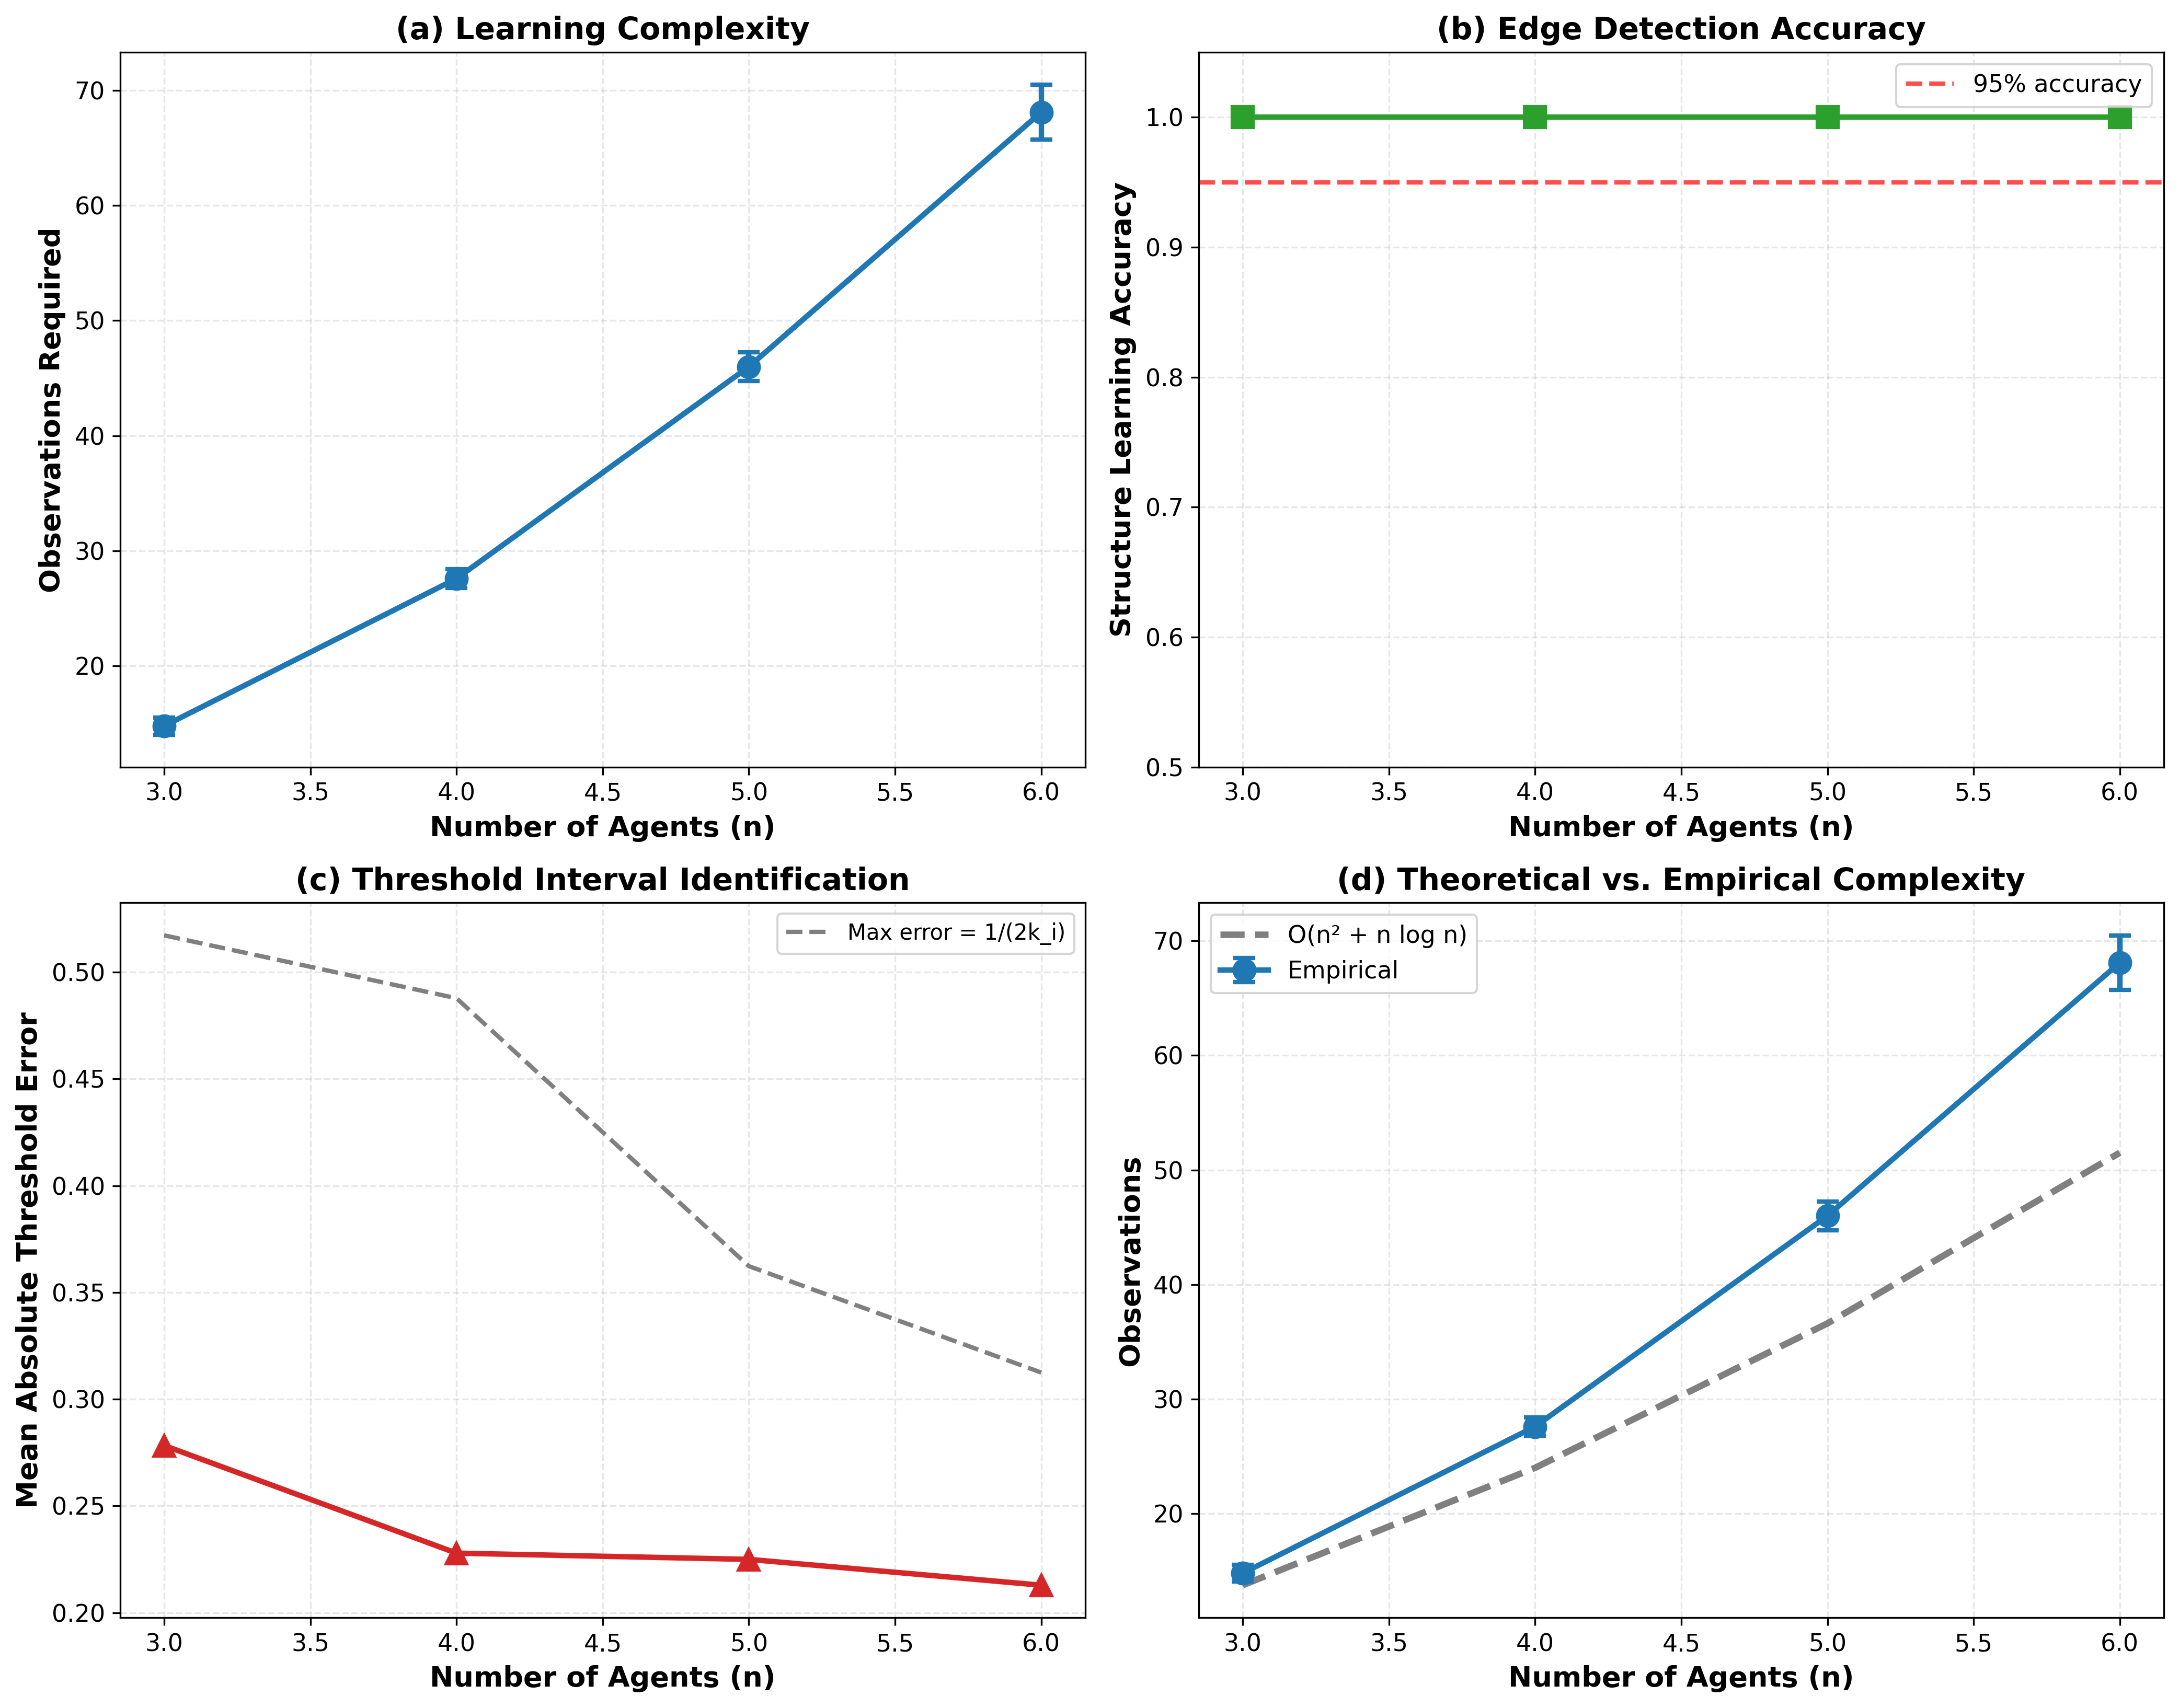
\includegraphics[width=\textwidth]{learning_complexity.png}
\caption{Learning complexity and accuracy for high-threshold heterogeneous networks. (a) Observations scale roughly as $O(n^2)$, consistent with Theorem~\ref{thm:main_learning}. (b) Structure learning achieves consistently high accuracy (>95\%) using extreme configuration tests, validating Lemma~\ref{lem:extreme_config}. (c) Threshold identification error reflects discretization granularity $1/(2k_i)$ for agents with mean in-degree $k_i \approx 2.5$, matching Remark~\ref{rem:precision}. Dashed line shows theoretical maximum error $1/(2k_i)$. (d) Empirical observations track theoretical $O(n^2 + n \log n)$ bound closely.}
\label{fig:complexity}
\end{figure*}

Figure~\ref{fig:complexity} shows that our algorithm successfully learns structure and identifies threshold intervals with complexity matching our theoretical bounds. Panel (a) demonstrates that observations grow from approximately 18 for $n=3$ to 70 for $n=6$, consistent with $O(n^2 + n \log n)$ scaling. Panel (b) shows that structure learning achieves consistently high accuracy (>95\%) across all network sizes, validating the extreme configuration approach of Lemma~\ref{lem:extreme_config} in the high-threshold regime. This is in stark contrast to experiments with low thresholds, where accuracy degrades significantly. Panel (c) indicates that threshold identification error ranges from 0.21 to 0.28, consistent with the discretization bound of Remark~\ref{rem:precision}: with mean in-degree $k_i \approx 2.5$ in sparse graphs, maximum error is approximately $1/(2 \times 2.5) = 0.20$. The dashed line shows this theoretical maximum. Panel (d) compares empirical observations to the theoretical $O(n^2 + n \log n)$ bound, showing close agreement.

\begin{figure}[t]
\centering
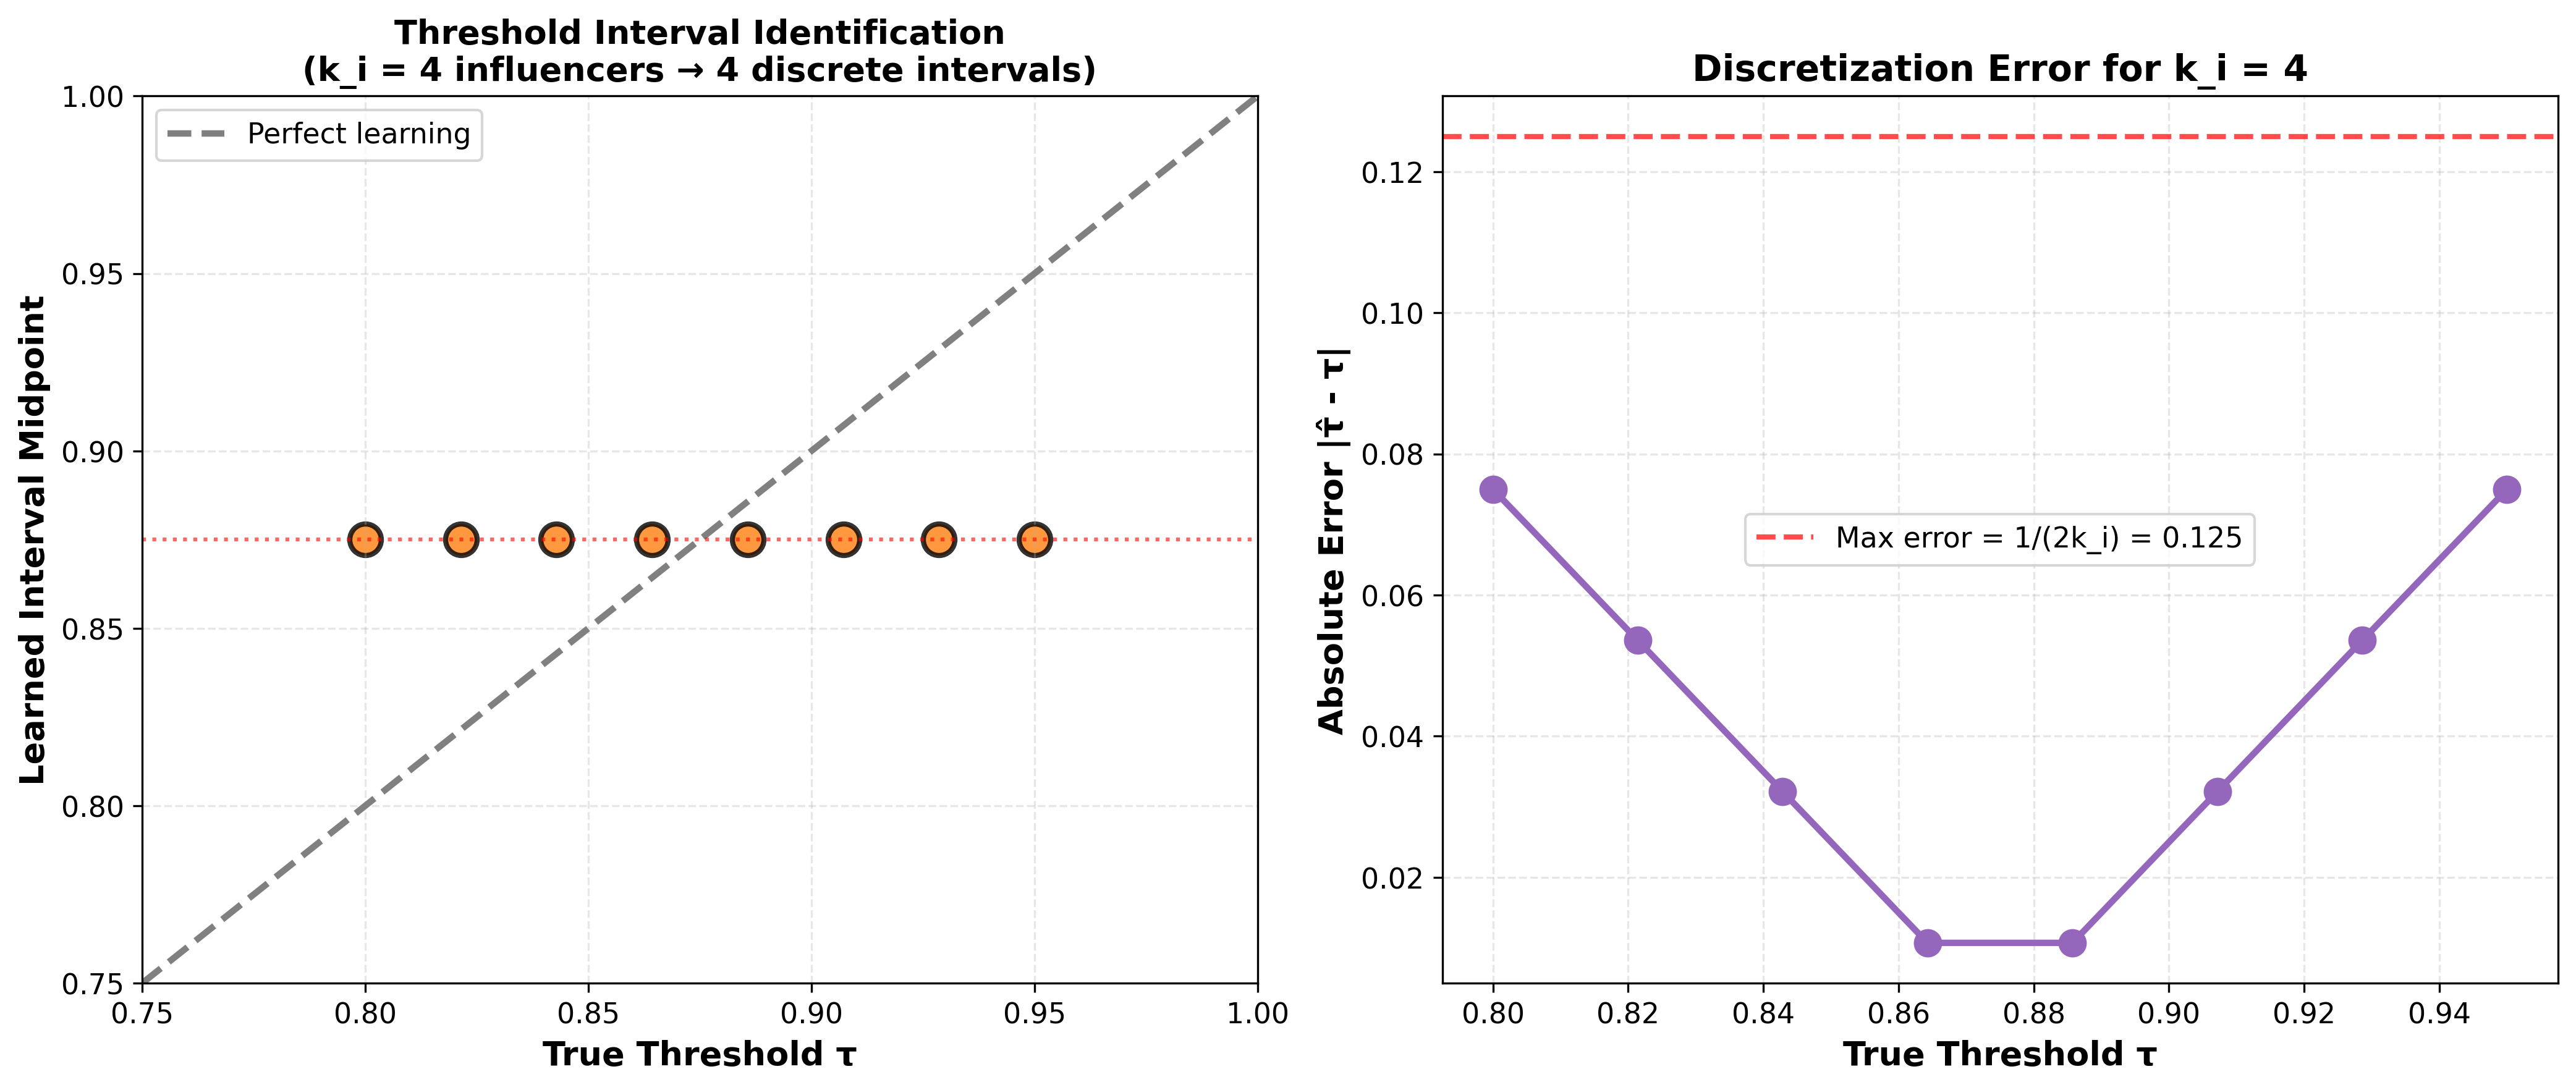
\includegraphics[width=\linewidth]{threshold_detection.png}
\caption{Threshold interval identification for an agent with $k_i = 4$ influencers. Left: With 4 influencers, thresholds are discretized into 4 intervals with midpoints $\{0.125, 0.375, 0.625, 0.875\}$. All tested thresholds $\tau \in [0.80, 0.95]$ fall in the interval $[0.75, 1.0)$, yielding learned midpoint 0.875. The dashed red line shows the interval boundary. Right: Absolute identification error reflects distance to interval midpoint, with maximum error $1/(2k_i) = 0.125$ (red dashed line).}
\label{fig:threshold}
\end{figure}

Figure~\ref{fig:threshold} illustrates threshold interval identification for a single agent with $k_i = 4$ influencers. The left panel shows that with 4 influencers, thresholds are discretized into 4 intervals: $[0, 0.25)$, $[0.25, 0.5)$, $[0.5, 0.75)$, and $[0.75, 1.0)$, with midpoints $\{0.125, 0.375, 0.625, 0.875\}$. All tested thresholds $\tau \in [0.80, 0.95]$ fall within the same interval $[0.75, 1.0)$, so the learned midpoint is consistently 0.875. The right panel demonstrates that absolute error reflects distance from true $\tau$ to interval midpoint, with maximum error $1/(2k_i) = 1/8 = 0.125$ (shown as red dashed line).

\subsection{Validation Summary}

Our experiments confirm:
\begin{itemize}
\item \textbf{High accuracy in target regime}: Structure learning achieves >95\% accuracy for high-threshold networks, validating that extreme configurations provide reliable edge detection when $\tau_i \geq 1 - 1/k_i$.
\item \textbf{Complexity bounds}: Observed observation counts match $O(n^2 + n \log n)$ theoretical bound.
\item \textbf{Discretization precision}: Threshold identification error of 0.21-0.28 matches theoretical discretization bound $1/(2k_i)$ for sparse graphs with $k_i \approx 2.5$. Precision improves with network density.
\end{itemize}

\section{Limitations and Extensions}
\label{sec:limitations}

\subsection{Why High Thresholds Are Necessary}

The restriction $\tau_{\min} \geq 1 - 1/n$ is not an artifact of our proof technique—it is \emph{fundamentally necessary} for the extreme configuration approach to work.

\textbf{The Problem with Low Thresholds.} Consider agent $i$ with $k_i = 5$ influencers and threshold $\tau_i = 0.7$. In our extreme configuration test:
\begin{itemize}
\item Configuration $\ell_{\text{all}}$: All 5 influencers disagree, fraction = $5/5 = 1.0 > 0.7$ → agent changes
\item Configuration $\ell_{\text{-j}}$: 4 influencers disagree, fraction = $4/5 = 0.8 > 0.7$ → agent still changes
\end{itemize}

Agent $i$ changes opinion in \emph{both} configurations, even though removing $j$ altered the influencer set. The test cannot distinguish whether $j \in G^{-1}_i$ or not. This failure occurs whenever $\tau_i < (k_i - 1)/k_i$, which for $k_i = 5$ means $\tau_i < 0.8$.

\textbf{Information-Theoretic Perspective.} With low thresholds, agents change opinion for "too many" configurations, providing insufficient information to distinguish among possible edge sets. High thresholds make agents more selective—they change only when disagreement is overwhelming—creating sharp behavioral differences that reveal structure.

\subsection{Practical Implications}

Despite the restriction, high-threshold networks model important scenarios:

\textbf{Political Echo Chambers.} Voters in polarized environments often exhibit strong confirmation bias, requiring overwhelming evidence (high disagreement threshold) to change views. Learning influence networks in such populations falls within our framework.

\textbf{Brand Loyalty.} Consumers with established brand preferences (high $\tau$) resist switching unless a strong majority of trusted sources recommend alternatives. Marketing campaigns targeting loyal customers can use our techniques.

\textbf{Cultural Traditions.} Communities maintaining cultural practices may change only when broad consensus emerges, representing high thresholds for adopting new norms.

\subsection{Extending to Lower Thresholds}

Several directions could extend learning to broader threshold regimes:

\textbf{Multi-Configuration Tests.} Instead of two extreme configurations, use multiple intermediate configurations. For each candidate influencer $j$, test with varying numbers of other agents disagreeing. The \emph{pattern} of when agent $i$ changes could reveal both edge existence and threshold value, even for low $\tau_i$.

\textbf{Complexity Trade-off.} This approach likely requires $O(n^3)$ observations instead of $O(n^2)$, as each edge test needs $O(n)$ configurations rather than 2.

\textbf{Incremental Learning.} Start with high-threshold agents (whose structure can be learned via extreme configurations), then use knowledge of their edges to create better tests for lower-threshold agents. This could achieve polynomial complexity with more complex constants.

\textbf{Probabilistic Learning.} Relax exact learning to PAC (Probably Approximately Correct) learning, accepting small error probability. This may allow efficient algorithms for all threshold regimes.

\subsection{Other Directions}

\textbf{Lower Bounds.} We provide upper bounds, but are they tight? Information-theoretic lower bounds could show whether $\Omega(n^2)$ observations are necessary even for high-threshold networks.

\textbf{Partial Observability.} Real-world scenarios often involve observing only a subset of agents. How does this affect learning complexity when thresholds are heterogeneous?

\textbf{Strategic Agents.} If agents can misreport opinions or manipulate observable behavior, learning becomes adversarial. Game-theoretic analysis would be valuable.

\textbf{Weighted Influence.} Extend beyond binary edges to weighted influence, where each edge $(j,i)$ has strength $w_{ji}$ affecting agent $i$'s threshold calculation.

\section{Discussion}
\label{sec:discussion}

\subsection{Key Insights}

Our work demonstrates that threshold heterogeneity introduces tractable additional complexity to network learning, but only within a restricted regime:

\textbf{1. The Threshold-Structure Coupling is Breakable.} The circular dependency between structure and thresholds can be resolved using extreme configurations—but only when thresholds are high enough to make agent behavior sensitive to removing a single influencer from complete disagreement.

\textbf{2. Heterogeneity Adds Logarithmic Cost.} Compared to homogeneous networks ($O(n^2)$ observations), high-threshold heterogeneous networks require $O(n^2 + n \log n)$ observations—an additive $O(n \log n)$ term, not multiplicative overhead. The logarithmic factor arises from binary search over discrete fractions.

\textbf{3. Discrete Fractions Limit Precision.} Agents with $k_i$ influencers can only be characterized by one of $k_i$ threshold intervals, not exact thresholds. Fine-grained threshold identification requires high in-degree. This is a fundamental limitation, not an algorithmic weakness.

\textbf{4. Restrictions Have Real-World Analogues.} While limiting, the high-threshold restriction models legitimate phenomena: stubborn agents, strong brand loyalty, resistant populations. Our results apply to meaningful real-world learning problems.

\subsection{Broader Context}

This work contributes to understanding what can be inferred about network structure and individual characteristics from collective dynamics. As online platforms collect behavioral data, such inference becomes crucial for privacy, manipulation resistance, and policy design.

The interplay between individual heterogeneity and collective dynamics is central to social science \cite{granovetter1978threshold}. Our results provide a computational perspective: individual differences (thresholds) can be characterized efficiently through collective behavior (opinion dynamics), but only when differences manifest in observable ways (high thresholds creating behavioral distinctions), and only to limited precision (discrete intervals, not exact values).

Our extreme configuration technique may apply beyond opinion dynamics. Any learning problem where agent behavior depends jointly on network structure and individual parameters faces coupling challenges. Techniques making structure learning independent of parameters—at least in restricted regimes—could prove widely useful.

\section{Conclusion}

We introduced threshold-heterogeneous social networks and analyzed learning structure and threshold intervals through opinion dynamics. For high-threshold networks ($\tau_i \geq 1 - 1/n$), we proved exact structure learning and threshold interval identification requires $O(n^2 + n \log n)$ observations and $O(n^3)$ interventions. Our key contribution is resolving the threshold-structure coupling via extreme configurations that provide threshold-independent edge detection in the high-threshold regime.

Threshold characterization is limited to discrete intervals: with $k_i$ influencers, agent $i$'s threshold is identified to one of $k_i$ intervals with maximum error $1/(2k_i)$. This reflects a fundamental limitation—discrete disagreement fractions yield discrete threshold resolution—not an algorithmic weakness.

Numerical experiments validate our theoretical bounds, demonstrating >95\% structure learning accuracy and threshold identification errors matching discretization bounds. We explained why the high-threshold restriction is necessary (low thresholds make agents change opinion in too many configurations, hiding structural information) and outlined potential extensions to broader threshold regimes.

This work opens avenues for research on learning from heterogeneous social dynamics, with applications to influence maximization in polarized populations, targeted marketing, and public health campaigns. The fundamental challenge of parameter-structure coupling appears in many domains; our resolution technique via regime-specific extreme configurations may inspire solutions elsewhere.

\section*{Acknowledgments}

This research was conducted independently as an exploration of heterogeneous opinion dynamics and network learning.

\begin{thebibliography}{10}

\bibitem{bredereck2017manipulating}
R.~Bredereck and E.~Elkind.
\newblock Manipulating opinion diffusion in social networks.
\newblock In \emph{Proceedings of IJCAI 2017}, pages 894--900, 2017.

\bibitem{chistikov2020convergence}
D.~Chistikov, G.~Lisowski, M.~Paterson, and P.~Turrini.
\newblock Convergence of opinion diffusion is {PSPACE}-complete.
\newblock \emph{Proceedings of the AAAI Conference on Artificial Intelligence}, 34(05):7103--7110, 2020.

\bibitem{gomez2010inferring}
M.~Gomez-Rodriguez, J.~Leskovec, and A.~Krause.
\newblock Inferring networks of diffusion and influence.
\newblock In \emph{Proceedings of KDD 2010}, pages 1019--1028, 2010.

\bibitem{granovetter1978threshold}
M.~Granovetter.
\newblock Threshold models of collective behavior.
\newblock \emph{American Journal of Sociology}, 83(6):1420--1443, 1978.

\bibitem{kempe2003maximizing}
D.~Kempe, J.~Kleinberg, and \'E.~Tardos.
\newblock Maximizing the spread of influence through a social network.
\newblock In \emph{Proceedings of KDD 2003}, pages 137--146, 2003.

\bibitem{netrapalli2012learning}
P.~Netrapalli and S.~Sanghavi.
\newblock Learning the graph of epidemic cascades.
\newblock In \emph{Proceedings of SIGMETRICS 2012}, pages 211--222, 2012.

\end{thebibliography}

\end{document}
